\documentclass[a4paper, 11pt, titlepage]{book}

% -----------------------------------------------------------------------
%                               PACKAGES
% -----------------------------------------------------------------------

\usepackage[paperheight=29.7cm,paperwidth=21cm,outer=1.5cm,inner=2.5cm,top=2cm,bottom=2cm]{geometry}
\usepackage[english]{babel}
\usepackage[utf8x]{inputenc}
\usepackage[T1]{fontenc}
\usepackage{titlesec}
\usepackage[titles]{tocloft}
\usepackage[nottoc]{tocbibind}
\usepackage{blindtext}
\usepackage{color}
\usepackage{epsfig}
\usepackage{plain}

\usepackage{setspace}
\singlespacing

\usepackage{fontawesome}
% Needed to have different sizes for fontawesome
\DeclareFontFamily{U}{fontawesomeOne}{}
\DeclareFontShape{U}{fontawesomeOne}{m}{n}
  {<-> FontAwesome--fontawesomeone}{}
\DeclareRobustCommand\FAone{\fontencoding{U}\fontfamily{fontawesomeOne}\selectfont}

% DRAFT background
\usepackage{background}
\backgroundsetup{contents=DRAFT}

% Code listing
%\usepackage{fontspec}
%\setmonofont[
%  Contextuals={Alternate}
%]{Fira Code}

\usepackage{listings}
%\usepackage{pxfonts}
\lstset{language=Python,
    basicstyle=\ttfamily,
    keywordstyle=\bfseries,
    showstringspaces=false,
    morekeywords={include, printf}
}

% Drop cap implementation
\usepackage{type1cm}
\usepackage{lettrine}

% Clickable references
\usepackage{hyperref}
\hypersetup{
    colorlinks,
    citecolor=black,
    filecolor=black,
    linkcolor=black,
    urlcolor=black
}

% Custom boxed/framed environments
\usepackage[framemethod=tikz]{mdframed}

% Font awesome
\usepackage{fontawesome}

% Black and white images
\usepackage{graphicx}

\usepackage{lipsum} % To be removed

% -----------------------------------------------------------------------
%                             FANCY TITLES
% -----------------------------------------------------------------------

\definecolor{gray75}{gray}{0.75}

% Fancy TOC
\renewcommand\cftchapfont{\normalfont}
\renewcommand\cftchappagefont{\normalfont}
\renewcommand{\cftchapafterpnum}{\vskip 5pt}
\renewcommand\cftsecafterpnum{\vskip 5pt}
\renewcommand\cftsubsecafterpnum{\vskip 5pt}
\setlength\cftbeforesecskip{0pt}
\setlength\cftbeforesubsecskip{0pt}

\AtBeginDocument{\renewcommand\contentsname{Table of Contents}}

\titleformat{\chapter}[display]
{}{\hfill\rule{.7\textwidth}{3pt}}{0pt}
{\hspace*{.3\textwidth}\huge\bfseries}[\addvspace{-1pt}]
\titleformat{name=\chapter,numberless}[display]
{}{\hfill\rule{.7\textwidth}{3pt}}{0pt}
{\hspace*{.3\textwidth}\huge\bfseries}[\addvspace{-1pt}]

% Fancy chapter titles
\newcommand{\hsp}{\hspace{20pt}}
\titleformat{\chapter}[hang]{\Huge\bfseries}{\thechapter\hsp\textcolor{gray75}{|}\hsp}{0pt}{\Huge\bfseries}

% -----------------------------------------------------------------------
%                               CODE BOX
% -----------------------------------------------------------------------

% Usage:
% \begin{code}
%	\begin{verbatim}
%		$ ls
%		
%		Applications	Desktop	...
%	\end{verbatim}
% \end{code}

\mdfdefinestyle{code}{
	leftmargin=10pt,
	rightmargin=10pt,
	innerleftmargin=15pt,
	middlelinecolor=gray75,
	middlelinewidth=2pt,
	frametitlerule=false,
	backgroundcolor=black!0.5!white,
	frametitle={\faCode \codeTitle},
	frametitlefont={\normalfont\sffamily\color{white}\hspace{-1em}},
	frametitlebackgroundcolor=gray75,
	nobreak,
}

\newenvironment{code}[1][Code]{
	\medskip
	\newcommand{\codeTitle}{~#1}
	\begin{mdframed}[style=code]
	}{
	\end{mdframed}
	\medskip
}

%\gls{ids} DEFINITION (SHORT)
%\glsxtrshort{ids} SHORT
%\glsxtrshortpl{ids} SHORT plural

\newacronym{ids}{IDS}{Intrusion Detection System}

\newacronym{sdn}{SDN}{Software Defined Network}

\newacronym{ml}{ML}{Machine Learning}

\newacronym{tcp}{TCP}{Transmission Control Protocol}

\newacronym{udp}{UDP}{User Datagram Protocol}

\newacronym{icmp}{ICMP}{Internet Control Message Protocol}

\newacronym{xss}{XSS}{Cross-site-scripting}

\newacronym{dos}{DoS}{Denial of Service}

\newacronym{ddos}{DDoS}{Distributed Denial of Service}

\newacronym{sql}{SQL}{Structured Query Language}

\newacronym{sqli}{SQLi}{SQL-Injection}

\newacronym{ai}{AI}{Artificial Intelligence}

\newacronym{tls}{TLS}{Transport Layer Security}

\newacronym{url}{URL}{Uniform Resource Locator}

\newacronym{html}{HTML}{HyperText Markup Language}

\newacronym{api}{API}{Application Programming Interface}

\newacronym{ip}{IP}{Internet Protocol}

\newacronym{ack}{ACK}{Acknowledge}

\newacronym{syn}{SYN}{Synchronize}

\newacronym{ietf}{IETF}{Internet Engineering Task Force}

\newacronym{fiat}{FIAT}{Forward Inter Arrival Time}

\newacronym{biat}{BIAT}{Backward Inter Arrival Time}

\newacronym{flowiat}{FlowIAT}{Flow Inter Arrival Time}

\newacronym{fbpsec}{FBPS}{Flow Bytes per Second}

\newacronym{fppsec}{FPPS}{Flow Packets per Second}

\newacronym{hids}{HIDS}{Host based Intrusion Detection System}

\newacronym{nids}{NIDS}{Network based Intrusion Detection System}

\newacronym{vm}{VM}{Virtual Machine}

\newacronym{tap}{TAP}{Test Access Port}

\newacronym{nic}{NIC}{Network Interface Card}

\newacronym{dpi}{DPI}{Deep Packet Inspection}

\newacronym{fpga}{FPGA}{Field Programmable Gate Array}

\newacronym{cic}{CIC}{Canadian Institute for Cybersecurity}

\newacronym{csv}{CSV}{Comma Separated Values}

\newacronym{pcap}{PCAP}{Packet Capture}

\newacronym{tp}{TP}{True Positive}

\newacronym{fp}{FP}{False Positive}

% -----------------------------------------------------------------------
%                               DOCUMENT
% -----------------------------------------------------------------------

\begin{document}

    % TITLE PAGE
    
    \pagenumbering{gobble}
    \pagestyle{plain}

\thispagestyle{empty}

\begin{center}
  \begin{figure}[h!]
    \centerline{
\psfig{file=assets/figures/marchio_unitrento_colore_it_202002_mod.eps, width=0.6\textwidth}}
  \end{figure}

  \vspace{2 cm} 

  \LARGE{Department of Information Engineering and Computer Science\\}

  \vspace{1 cm} 
  \Large{Bachelor’s Degree in\\
    Information and Communications Engineering
  }

  \vspace{2 cm} 
  \Large\textsc{Final Dissertation\\} 
  \vspace{1 cm} 
  \Huge\textsc{Machine Learning for Virtualized-Network Intrusion Detection System}


  \vspace{2 cm} 
  \begin{tabular*}{\textwidth}{ c @{\extracolsep{\fill}} c }
  \Large{Supervisor} & \Large{Student}\\
  \Large{Prof. Fabrizio Granelli}& \Large{Giovanni Baccichet}\\
  \end{tabular*}

  \vspace{2 cm} 

  \Large{Academic year  2020/21}
  
\end{center}
    \clearpage

    % ABSTRACT

    \thispagestyle{empty}

{\bf\Huge Abstract}

\vspace{1cm}

\lipsum[1-3] \\ \faGithub

\vspace{1cm}

{\bf\Huge Keywords}

\vspace{1cm}

\begin{itemize}
    \item Cyber Security
    \item Intrusion Detection System
    \item Machine Learning
    \item Software Defined Networks
    \item Themis
\end{itemize}
    \clearpage

    % TOC

    \mainmatter
    \tableofcontents
    %\listoffigures
    %\listoftables
    \clearpage

    % CHAPTER 1 - Introduction

    \chapter{Introduction}
\label{chap:intro}

\lettrine[lines=3, findent=3pt, nindent=0pt]{G}{lobal} village was the term coined in the 1960s by the Canadian thinker H. Marshall McLuhan \cite{mcluhan1962} to describe the society after the birth of mass media: all parts of the World were brought together by the communication abilities given by technological advancement. \\
Nowadays, with broad adoption of digital technologies, mass-communication represents the foundation of modern society, leading to concerns about privacy and security.



%----------------------------------------------------
% PROBLEM
%----------------------------------------------------

\section{Problem}
\label{sec:problem}

The evolution of cyber-attack techniques, becoming more sophisticated than ever, poses a critical challenge in accurately and reliably detecting intrusions.\\ The first \gls{ids} was proposed in 1980 \cite{Andreson1980} and since then the industry has arisen, but modern \glsxtrshortpl{ids} aren't still perfect and suffer mainly from two problems:
\begin{itemize}
    \item[\faCaretRight] \textit{False-alarm rate}: generating too many alerts for nonthreatening situations raises the burden for security analysts, and can cause harmful attacks to be ignored;
    \item[\faCaretRight] \textit{Unknown attack detection}: attack variants and novel attacks emerge constantly and more and more frequently, hence the need of being able to detect unknown attacks. Some \gls{ids} rely on the signatures of known attacks and cannot identify new threats \cite{Hodo2017}.
\end{itemize}
Researchers in this filed aim at having a high accuracy of detection and low false alarm rate. \\
If provided with sufficient training data, machine learning algorithms can detect both attack variants and novel ones \cite{Hodo2017}. Another perk brought by machine learning models is that they do not rely heavily on domain knowledge, and so have a more lightweight design \cite{Khraisat2019}. \\ With that in mind, in order to achieve well grounded results, it is necessary to know which network features represent which attack \cite{Iglesias2015} and what data is sustainable for detecting certain types of attacks. Furthermore a comprehensive analysis of machine learning algorithms is needed for identifying the most suitable one for the implementation \cite{Liu2019}, alongside the dataset needed for its training \cite{Sharafaldin2019}.


%----------------------------------------------------
% GOAL
%----------------------------------------------------

\section{Objectives}
\label{sec:objectives}

In order to solve the problems displayed above, it would be helpful to use machine learning algorithms to improve the accuracy of threats-detection, with flexible and dynamic monitoring of the network. This project can be broken into the following milestones:

\begin{enumerate}
    \item Setting up a virtualized environment for testing purposes (this has to be scalable, to represent a realistic scenario);
    \item Choosing a \gls{sdn} Controller on which running, as an application, a monitoring software to gather data about network flow;
    \item Identifying useful traffic features and extracting them with the chosen \gls{sdn} Controller;
    \item Choosing a machine learning algorithm suitable for this use;
    \item Performing machine learning classification of the above extracted traffic features to detect malicious traffic;
    \item Evaluating the performance of the \gls{ids} using an appropriate dataset.
\end{enumerate}
Practically the first three points concern building a network monitor capable of saving traffic data. Such data will be analyzed by the software developed in the last three points.

%----------------------------------------------------
% DELIMITATION
%----------------------------------------------------

\subsection{Delimitation}
\label{subsec:delimitation}

\faEdit \quad \textbf{To be defined after the methodology chapter.} \\

\textcolor{dimgray}{\lipsum[1-2]}



    % CHAPTER 2 - State of the Art

    \chapter{State of the Art}
\label{chap:state-of-the-art}

\lettrine[lines=3, findent=3pt, nindent=0pt]{T}{his} chapter rounds out the theoretical background and technologies used in the project and discussed in the following: beginning with how network traffic is made ad how to characterize malicious activities, it will then be discussed Software Defined Networking as an industry standard and then \gls{ml} will be introduced, with particular emphasis on Intrusion Detection applications of \textit{Deep Learning}. The reader should here be provided with sufficient knowledge to understand chapters \ref{chap:methodology}, \ref{chap:results} and \ref{chap:conclusions}.

%----------------------------------------------------
% NETWORK TRAFFIC
%----------------------------------------------------

\section{Network Traffic}
\label{sec:network-traffic}

\textit{Network Traffic} is the amount of data that passes through a network at a given time, and it represents the starting point to the project. \\ Network architecture was thought to be modular and explicit, to ensure that modifications made to a single component were transparent to the rest of the system. This modularization is represented by \textit{network protocols} being separated into different layers: each layer has a precise task. In 1960s the \textit{U.S. Department of Defense} designed the \textit{TCP/IP} model, which is now the \textit{de facto} standard for protocols stack. Network security should be addressed at each TCP/IP network layer for different vulnerabilities and attack types \cite{Zaman2009}.

\begin{figure}[h!]
    \centering
    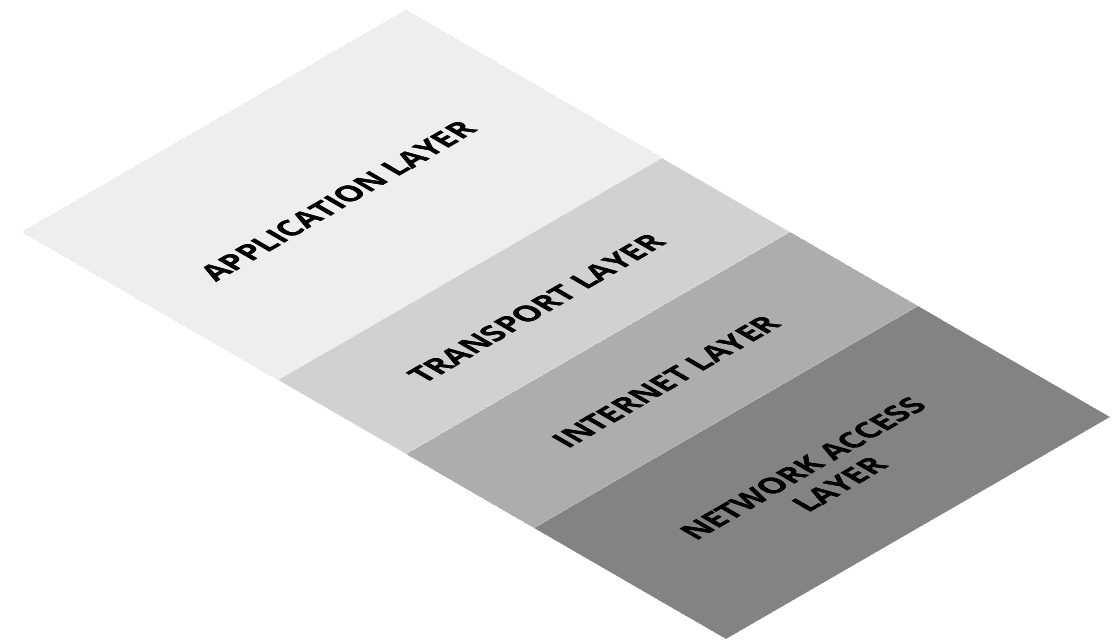
\includegraphics[scale=0.23]{figures/TCP_IP Stack.png}
    \caption{Internet protocol suite: TCP/IP Stack}
    \label{fig:TCP/IP-stack}
\end{figure}

TCP/IP stack is composed of 4 layers, representing from the physical connection (\textit{Network Access Layer}) to the user interface (\textit{Application Layer}). \\ The most relevant layer for this project is the third one: \textit{Transport Layer}, also called \textit{Host to Host Layer} is responsible for end-to-end communication and error-free delivery of data. It shields the upper-layer applications from the complexities of data. The main protocols used in this layer are:

\begin{itemize}
    \item[\faCaretRight] \gls{tcp}: provides reliable and error-free communication between end systems. It also has acknowledgement features and a flow control system. This protocol has a lot of overhead due to its features;
    \item[\faCaretRight] \gls{udp}: unlikely \gls{tcp}, this protocol doesn't ensure a reliable connection between points, but it is very cost effective and lightweight.
\end{itemize}
Network packets are encapsulated in either a \textit{TCP segment} or a \textit{UDP datagram}. Another relevant protocol that will be used is \gls{icmp}, belonging to the second layer (\textit{Internet Layer}): it s responsible for providing hosts with information about network problems. Because of the particular design of network architecture, in which one layer acts as an intermediate between the layer above and the one below, when trying to characterize the traffic, looking only at these latter protocols can be sufficient \cite{Iglesias2015}.

%----------------------------------------------------
% SOFTWARE DEFINED NETWORKING
%----------------------------------------------------

\subsection{Software Defined Networking}
\label{subsec:sdn}

Follows a brief introduction on \gls{sdn} as an industry standard, now widely available also in consumer-grade equipment. These notions will be useful to comprehend section \ref{subsec:traffic-characterization}. \\
\gls{sdn} technology is an approach to network management that enables dynamic and efficient network configuration with the aim of improving network performance and monitoring. It was first issued by \gls{ietf} in the 2000s and since its refinement it was associated with \textit{OpenFlow protocol}, although nowadays it isn't anymore an exclusive solution. In the \gls{sdn} paradigm the network architecture consists fo three planes: \textit{data plane} (that forwards traffic according to the decisions made by the control plane), \textit{control plane} (that decides how to handle network traffic) and \textit{application plane} \cite{Kreutz2015}.

\begin{figure}[h!]
    \centering
    \begin{tikzpicture}[scale=.45,every node/.style={minimum size=1cm},on grid]
            
        %slanting: production of a set of n 'laminae' to be piled up. N=number of grids.
        \begin{scope}[
                yshift=-83,every node/.append style={
                yslant=0.5,xslant=-1},yslant=0.5,xslant=-1
                ]
            % opacity to prevent graphical interference
            \fill[white,fill opacity=0.9] (0,0) rectangle (5,5);
            \draw (2.5,2.5) node {\fontsize{50}{60} \faRandom};
            \draw[black,very thick] (0,0) rectangle (5,5);%marking borders
            %Idem as above, for the n-th grid:
        \end{scope}
            
        \begin{scope}[
            yshift=0,every node/.append style={
                yslant=0.5,xslant=-1},yslant=0.5,xslant=-1
                         ]
            \fill[white,fill opacity=.9] (0,0) rectangle (5,5);
            \draw[black,very thick] (0,0) rectangle (5,5);
            \draw (2.5,2.5) node {\fontsize{50}{60} \faServer};
        \end{scope}
            
        \begin{scope}[
            yshift=90,every node/.append style={
            yslant=0.5,xslant=-1},yslant=0.5,xslant=-1
                         ]
            \fill[white,fill opacity=.9] (0,0) rectangle (5,5);
            \draw (2.5,2.5) node {\fontsize{50}{60} \faTv};
            \draw[black,dashed] (0,0) rectangle (5,5);
        \end{scope}
    
        %putting arrows and labels:
        \draw[-latex,thick] (6,4) node[right]{$\mathsf{Control\; Plane}$}
             to[out=180,in=90] (3.5,2.5);
    
        \draw[-latex,thick](6,1)node[right]{$\mathsf{Data\; Plane}$}
             to[out=180,in=90] (3.5,-0.5);
    
        \draw[-latex,thick](6,7)node[right]{$\mathsf{Application\; Plane}$}
            to[out=180,in=90] (3.5,5.5);
        
    \end{tikzpicture}
    \caption{\gls{sdn} paradigm}
    \label{fig:sdn-paradigm}
\end{figure}
The bottom plane is made up of \gls{sdn}-enabled switches, that send routing request to the above plane, instead of calculating routing rules by themselves when receiving new \textit{flows}, then the control plane calculates paths for the requests and assigns the routing rules in compliance with the applications in the top plane \cite{Xu2017}. A \textit{flow} is the set of packets within a time window, which reflects the network environment \cite{Liu2019}. The \textit{controller} exercises direct control over the state in the data plane elements via well-defined \glsplural{api}, such as OpenFlow. An OpenFlow switch has one or more tables of packet-handling rules (flow table). Each rule matches a subset of the traffic and performs certain actions on the traffic. Depending on the rules installed by a controller application, an OpenFlow switch can - instructed by the controller - behave like a router, switch, firewall, or perform other roles and this is the meaning of \textit{Software Defined} in \gls{sdn}.

%----------------------------------------------------
% SOFTWARE DEFINED NETWORKING
%----------------------------------------------------

\subsubsection{SDN Controller}
\label{ssubsec:sdn-controller}

%See paper \cite{Zhu2019} and \cite{Bondkovskii2016} \\
The \textit{controller} in the control plane is the fundamental element used for all operations of data plane management. Hence, the performance and capabilities of the controller itself are extremely important and in this project its \glsplural{api} will be needed for building a network traffic monitor (and such data will be use to recognize any possible attack). In \cite{Bondkovskii2016} and \cite{Zhu2019} different controllers are compared based on benchmarks, programming languages, documentation and other parameters (\textit{Northbound \glsxtrshort{api}}, \textit{Southbound \glsxtrshort{api}}, \textit{Multithreading}, \textit{Modularity}, etc). \\ In light of this, the controller of choice for the project will be \textit{Ryu Controller}: it outperformed other controllers on almost every benchmark, it has a very well made documentation \cite{RyuDoc} and it supports OpenFlow protocol up to version 1.5.

%----------------------------------------------------
% TRAFFIC CHARACTERIZATION
%----------------------------------------------------

%See paper \cite{Iglesias2015}, \cite{Sharafaldin2019} and \cite{icissp17} and \cite{Xu2017} and \cite{Dainotti2006} and \cite{Wijesinghe2015}

\subsection{Traffic Characterization}
\label{subsec:traffic-characterization}

Anomaly detection in communication networks provides the basis for uncovering misconfigurations, network failures and potential threats. Resource and time constraints create the need of restricting to a limited number of features the traffic characterization and task detection. Limiting the resources spent for the observation and the analysis of such data, also improves the quality of the detection, since trivial and redundant data will not be considered. There are two different methodologies to characterize network traffic: \textit{packet inspection} and \textit{flow-based characterization}. The first one consists of inspecting each network packet; it is very resource consuming and not always allowed since the payload can be encrypted. On the other hand, the second one is less precise, but much more cost effective and lightweight \cite{Alaidaros2017}. Machine learning methodologies can improve the detection rate of \textit{flow-based characterization} \cite{Iglesias2015}: this makes it a reliable go-to. In \cite{icissp17} \textit{time-related} features are suggested to characterize traffic with ease:
\begin{itemize}
    \item[\faCaretRight] \textit{Active}: duration of sending packets before idle;
    \item[\faCaretRight] \gls{biat}: time between two packets sent backward;
    \item[\faCaretRight] \textit{Duration}: duration of the considered flow.
    \item[\faCaretRight] \gls{fbpsec}: bytes sent per second in either direction;
    \item[\faCaretRight] \gls{flowiat}: time between two packets sent in either direction; 
    \item[\faCaretRight] \gls{fppsec}: packets sent per second in either direction;
    \item[\faCaretRight] \gls{fiat}: time between two packets sent forward; 
    \item[\faCaretRight] \textit{Idle}: amount of time the flow was idling before becoming active;
\end{itemize}
For all the features (extracted using \textit{Ryu Controller}) also the respective mean, minimum, maximum and standard deviation are calculated and so the above bullet list really represents groups of features, that are not exhaustive\footnote{See appendix \ref{app:net-features} for a table comparing attacks and features} of all possible features related to cyber-attacks. Another high-level semantic information of traffic can be a \textit{session}: a packet sequence combined on the basis of a network information 5-tuple (\textit{source ip}, \textit{destination ip}, \textit{source port}, \textit{destination port} and \textit{protocol}) \cite{Liu2019}.
\textcolor{dimgray}{\lipsum[1-3]}

%----------------------------------------------------
% MALICIOUS TRAFFIC
%----------------------------------------------------

\subsection{Malicious Network Traffic}
\label{subsec:malicious-traffic}

An \textit{intrusion} can be defined as an attempt to access information about computer systems or to damage system operation in an illegal or unauthorized manner \cite{Liu2019}, hence it will be considered \textit{malicious traffic} the entirety of network traffic generated by such operations. \\
The classes of malicious traffic analyzed in this work are the following:

\begin{itemize}
    \item[\faCaretRight] \textit{Botnet}: a botnet is a number of Internet connected devices, used to perform various tasks, from stealing data, to spam, or to practice \gls{ddos} attacks. Automated infection tools can also be used to scan for and compromise suitable zombie systems \cite{icissp18} and \cite[p.~250]{Sharafaldin2019};
    \item[\faCaretRight] \textit{Bruteforce}: this kind of attack is one of the most popular and it can be used to guess passwords or \glsxtrshortpl{url} (in order to discover hidden contents in web applications). It can be defined as an hint and try attack, that corresponds of trying every possible key on a piece of ciphertext until an intelligible translation into plaintext is obtained \cite{icissp18} and \cite[p.~43]{Sharafaldin2019};
    \item[\faCaretRight] \gls{xss}: this kind of vulnerability can typically be found in web applications. An \gls{xss} attack consist of injecting client-side scripts into \glsxtrshort{html} content of web pages, that can be viewed by other users and aims to gain elevated access privileges to sensitive data belong- ing to other sites \cite[p.~387]{Sharafaldin2019};
    \item[\faCaretRight] \gls{dos}: the objective of this attack is to exhaust some critical resources associated with the target service, denying or preventing legitimate users to access the system or the network \cite[p.~241]{Sharafaldin2019};
    \item[\faCaretRight] \gls{ddos}: unlike the previous type of attack, the incoming traffic flooding the victim is obtained from many different sources. This effectively makes it impossible to stop the attack simply by blocking a single source and guarantees much more bandwidth to the attacker \cite[p.~241]{Sharafaldin2019};
    \item[\faCaretRight] \textit{Heartbleed}: this particular attack exploits a bug in the OpenSSL cryptography library, widely used implementation of the \gls{tls} protocol. It was discovered in 2014 and allowed to expose significant amounts of memory on the vulnerable system \cite{Carvalho2014}, \cite{icissp18}, \cite{Stallings2014} and \cite[p.~706]{Sharafaldin2019};
    \item[\faCaretRight] \textit{Port Scanning}: this occurs when an attacker sends probe packets to gather intelligence information about the infrastructure, based on the responses received \cite{icissp18};
    \item[\faCaretRight] \gls{sqli}: it is one of the most prevalent and dangerous network-based security threats that uses malicious database queries to extract bulk data from the latter; this can occur, for example, through badly projected forms on web pages \cite[p.~163]{Sharafaldin2019}.
\end{itemize}
This list isn't exhaustive of all possible network violations, but these are the attacks contained in the dataset\footnote{See section \ref{subsec:datasets-for-evaluation}} used for the evaluation. Regarding the characterization of said violations, a comprehensive list of network features and related attacks can be found in appendix \ref{app:net-features}.
\textcolor{dimgray}{\lipsum[1]}

%----------------------------------------------------
% INTRUSION DETECTION SYSTEMS
%----------------------------------------------------

\section{Intrusion Detection Systems}
\label{sec:intrusion-detection-system}

An \gls{ids} is a piece of software put in place to monitor computer networks: by analyzing patterns of captured data from a network, it helps to detect threats. \glsplural{ids} are placed strategically on a network to detect malicious packets going through the traffic \cite{Hodo2017}. Figure \ref{fig:IDS-model} displays a possible implementation of an \gls{ids} in a network.

\begin{figure}[h!]
        \centering
        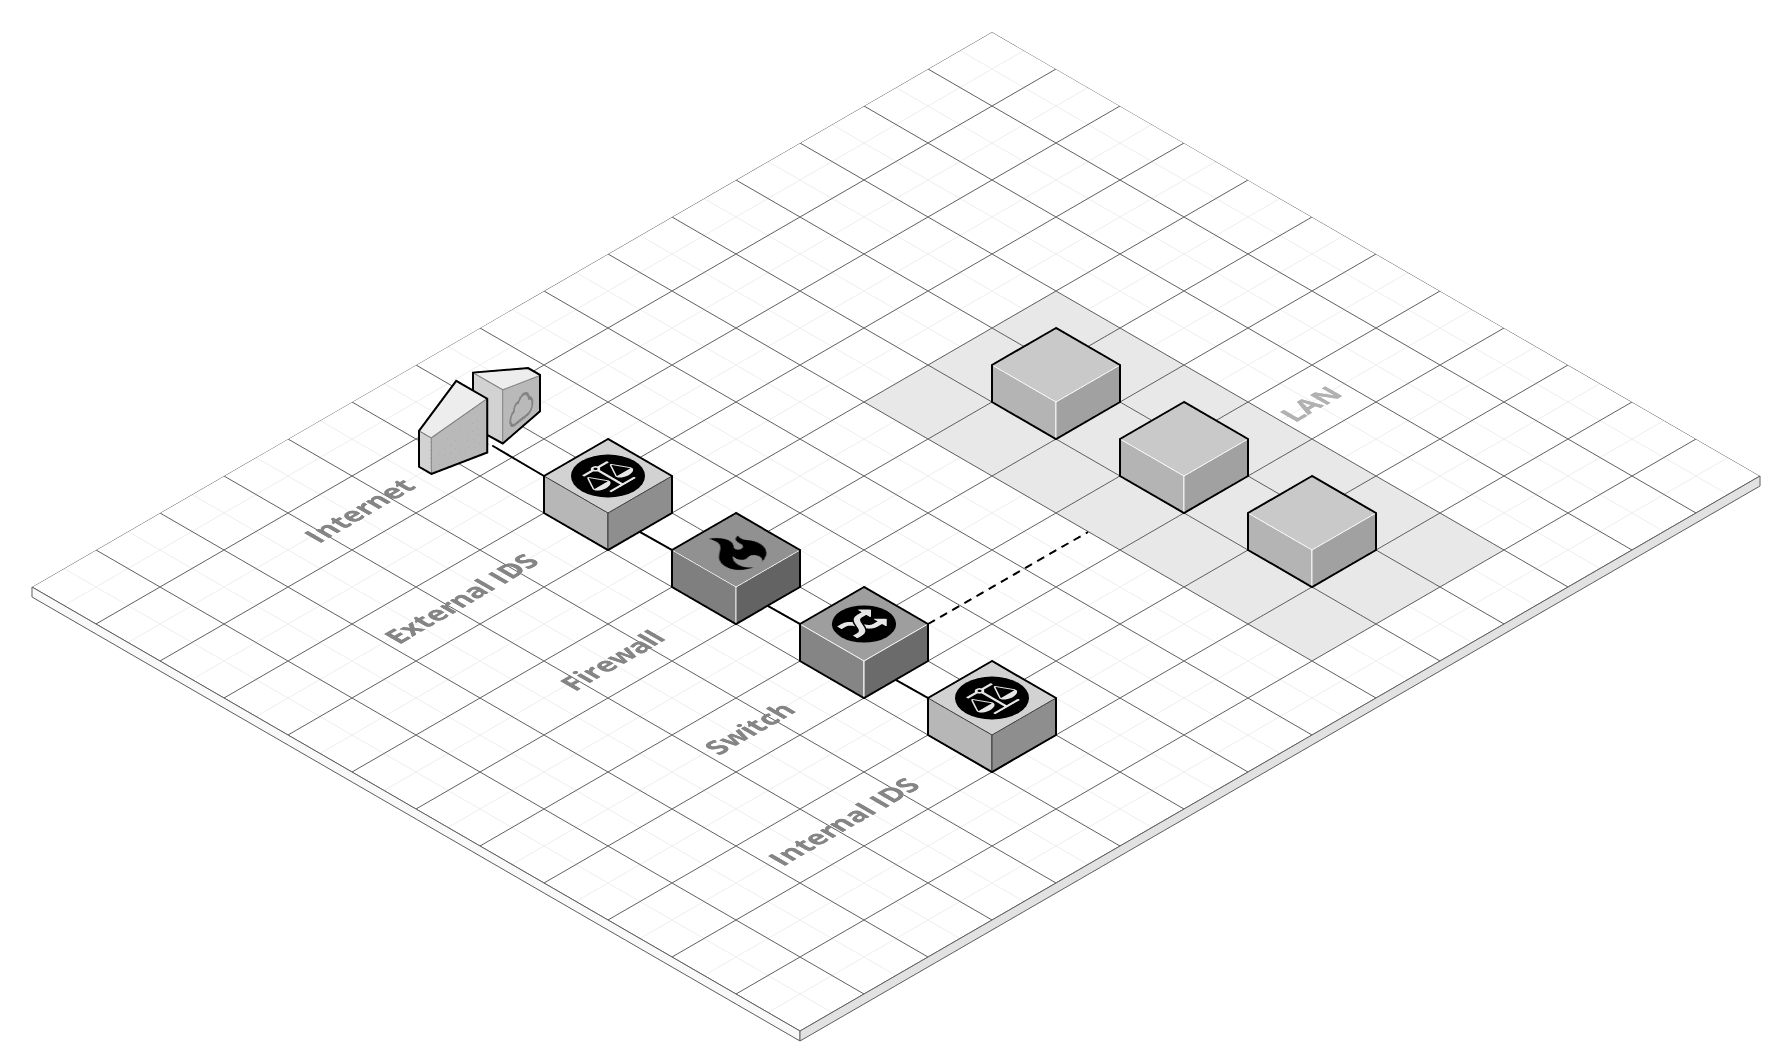
\includegraphics[scale=0.2]{figures/Intrusion Detection System Model.png}
        \caption{Intrusion Detection System Model}
        \label{fig:IDS-model}
\end{figure}
The functions demanded to an \gls{ids} are basically to detect and to give information about threats, such as those discussed in \ref{subsec:malicious-traffic}. There is a variety of implementations of \glsplural{ids} and detection models, which are briefly discussed in the following section \ref{subsec:taxonomy-ids}.

%----------------------------------------------------
% TAXONOMY OF INTRUSION DETECTION SYSTEMS
%----------------------------------------------------

%See paper \cite{Liu2019}

\subsection{Taxonomy of Intrusion Detection Systems}
\label{subsec:taxonomy-ids}

Different researchers have developed multiple classification representations of \glsplural{ids}: they can be classified by source of data (either host or network based, or both), by detection technique (anomaly based, signature based, or can use artificial intelligence). A good summary of the taxonomy and methodologies used can be \cite{Hodo2017} and \cite{Liu2019}, which cover also \gls{ml} applied to \gls{ids}.

\subsubsection{HIDS and NIDS}
\label{subsubsec:hids-nids}

As mentioned above, \glsplural{ids} can fall into two different categories: \gls{hids} was the first type to be implemented \cite{Debar1999} and consists in an application that, once installed on a host machine, analyzes and monitors all the network activities related to such computer. The traffic activities gathered are called \textit{audit trails}. There is one main advantage in using this typology of \gls{ids}: being able to detect threat before sending and receiving data. Its main disadvantage is that in order to monitor the whole network, it would be necessary to install that piece of software in every host \cite{Hodo2017}, resulting in occupying resources and in depending on the reliability of the single host \cite{Liu2019}. \\ On the other hand a \gls{nids} can be considered as a strong deterrence against outside intruders, in fact it is placed at specific points on the network (usually deployed on major hosts or switches \cite{Liu2019}), monitoring the network links. The main disadvantage is its weakness in detecting attacks generated inside the network \cite{Hodo2017}, because of its nature, it monitors only specific network segments \cite{Liu2019}.

\subsubsection{Anomaly-based Detection}
\label{subsubsec:anomaly-detection}

This is a behavioural-based technique that observes changes in normal activity by building, over a period of time, a profile of the monitored system. The main advantage of this technique is that it allows for unknown attack detection (since it knows what normal traffic looks like). \\ According to \cite{Hodo2017}, there are two categories of Anomaly Detection: \textit{self-learning} and \textit{programmed}. The first one is also divided in two branches: \textit{time series model}, that considers a sequence of observations in order of succession occurring in intervals of uniformity, heavily relying on probability analysis, and machine learning; the latter  will be discussed in section \ref{sec:machine-learning}. \\ Instead, a programmed model (divided into \textit{threshold}, \textit{simple rule based} and \textit{statistical models}) consists of a system that needs an external entity for learning how to detect changes in behaviour.

\subsubsection{Signature-based Detection}
\label{subsubsec:signature-detection}

Signature-based Detection uses a set of pre-defined rules to match the patterns in the network traffic \cite{Hodo2017}. Its selling point is the low false-positive detection ratio, whereas its main drawback is the detection capabilities: stuck to the database of known attacks. For this reason this type of detection will not be considered in this project.

%----------------------------------------------------
% DETECTION RATES
%----------------------------------------------------

\subsection{Detection rates and base-rate fallacy}
\label{subsec:detection-rates}

Understanding how accurate is an \gls{ids}, or a detection model is fundamental for making the right choices during the development. Moreover, understanding which parameters are important and which may only \textit{seem} to be important. These values can be obtained using some probability calculation and statistics. In \cite{Axelsson2000} the author used the \textit{base-rate fallacy}, one of the cornerstones of Bayesian statistics. A similar concept was applied in \cite{Liu2019} for evaluating the effectiveness of a \gls{ml} algorithm. The parameters needed to evaluate the \textit{effectiveness} of an \gls{ids} are:
\begin{itemize}
    \item[\faCaretRight] \textit{True Positive rate}: namely, a measure of attacks rightly classified as threats. It is represented by the conditional probability of an alarm triggered $A$ given that there has been an intrusion $I$, so $P(A|I)$;
    \item[\faCaretRight] \textit{False Positive rate}: also called \textit{False Alarm rate}, it indicates a measure of normal events, misclassified as attacks. It it the conditional probability of an attack being detected, given that there wasn't any, so $P(A|\neg I)$.
\end{itemize}
Recalling the \textit{conditional probability} of $A$, given that $B$ has occurred:
\begin{equation}
    P(A|B)=\frac{P(A)\cdot P(B|A)}{P(B)}
    \label{eq:conditional-prob}
\end{equation}
And the \textit{Bayes Theorem}:
\begin{equation}
    P(A|B)=\frac{P(A)\cdot P(B|A)}{\sum_{i=1}^nP(A_i)\cdot P(B|A_i)}
    \label{eq:Bayes-th}
\end{equation}
It is now possible to make some assumptions on what the ideal \gls{ids} should aim to: achieving substantial values of \textit{Bayesian Detection rate} $P(I|A)$, minimizing $P(A|\neg I)$, in other words, the false alarms. Considering \ref{eq:Bayes-th}, the Bayesian Detection rate can be calculated:
\begin{equation}
    P(I|A)=\frac{P(I)\cdot P(A|I)}{P(I)\cdot P(A|I)+ P(\neg I)\cdot P(A|\neg I)}
    \label{eq:Bayesian-detection-rate}
\end{equation}
Equation \ref{eq:Bayesian-detection-rate} refers to the probability that an alarm really indicates an intrusion: it is noticeable now that the limiting-factor in an \gls{ids} is not the ability to identify the behaviour correctly as a threat, rather its ability to suppress false alarms: the factor concerning the detection rate is overshadowed by the factor governing the false alarm rate, since intrusions don't happen so often, $P(I)<P(\neg I)$, but it is also true that $P(I)+P(\neg I)=1$; giving some examples for further explanation, assuming $P(I)=2\cdot 10^{-5}\Rightarrow P(\neg I)=0.99998$, and now the discrepancy is evident \cite{Axelsson2000}. \\ This demonstrates that, during the development of an \gls{ids} it is necessary to keep an eye on the \textit{False Positive rate}, in order to be as effective as possible.

%----------------------------------------------------
% DATASETS FOR INTRUSION DETECTION SYSTEMS
%----------------------------------------------------

\subsection{Datasets for Intrusion Detection Evaluation}
\label{subsec:datasets-for-evaluation}

See paper \cite{icissp18}, \cite{Khraisat2019} and \cite{Leevy2020} \lipsum[1-3]

\begin{center}
    \begin{chronology}*[2]{1998}{2020}{\textwidth}
        \event{1999}{DARPA \\ KDD}
        \event{2002}{DEFCON}
        \event{2016}{CAIDA}
        \event{2005}{LBNL}
        \event{2009}{CDX \\ Twente \\ Kyoto}
        \event{2011}{UMASS}
        \event{2012}{ISCX2012}
        \event{2013}{ADFA}
        \event{2017}{CICIDS2017}
        \event{2018}{CICIDS2018}
    \end{chronology}
\end{center}

%----------------------------------------------------
% MACHINE LEARNING
%----------------------------------------------------

\section{Machine Learning}
\label{sec:machine-learning}

See paper \cite{Khraisat2019} and \cite{Hodo2017} \\

\lipsum \\
Discussed in \ref{sec:machine-learning}

%----------------------------------------------------
% MACHINE LEARNING ALGORITHMS
%----------------------------------------------------

\subsection{Machine Learning Algorithms}
\label{subsec:ml-algorithms}

\lipsum

%----------------------------------------------------
% DEEP LEARNING
%----------------------------------------------------

\subsection{Deep Learning}
\label{subsec:deep-learning}

\lipsum

%----------------------------------------------------
% MACHINE LEARNING LIBRARIES
%----------------------------------------------------

\subsection{Machine Learning Libraries}
\label{subsec:ml-libraries}

\lipsum[1-3]

    % CHAPTER 3 - Methodology

    \chapter{Methodology}

    % CHAPTER 4 - Results

    \chapter{Results}
\label{chap:results}

    % CHAPTER 5 - Conclusions

    \chapter{Conclusions}

    % BIBLIOGRAPHY

    \bibliographystyle{plain}
    \bibliography{bibliography}
    \pagenumbering{roman}

    % ACRONYMS

    \printnoidxglossaries

    % APPENDICES

    \appendix
    \part*{Appendices}
    \chapter{Abbreviations}

\lipsum[1-10]
    \newpage
\thispagestyle{empty}

\vspace*{\fill}
    \begin{center}
      {\fontsize{50}{60} \faRecycle}\\[0.5cm]
      {\Large Printed on recycled paper}\\[0.4cm]
      {\color{gray75} Each tonne of recycled fibre that displaces a tonne of virgin fibre \\ saves about 24 trees, reducing wastewater generation (33\%), air \\ particulate emissions (28\%) and solid waste (54\%)}\\[0.4cm]
    \end{center}
    \vspace*{\fill}

\end{document}